%=================================================================
\section{Introduction}\label{sec-intro}

Nowadays,
data has increased in a large scale
in various fields such as Internet,
business,
telecommunication,
and biosciences.
Big data is refered to describe
the large and distributed
nature of the data sets,
this area has recently become a focus of scholarship.
Doug Laney~\cite{laney01controlling3v} defined challenges
and  brought about  increased data
with a 3Vs model,
i.e., Volume,
Velocity,
and Variety.
Volume means the size of the data that becomes increasingly big;
Velocity means data collection and analysis 
must be rapidly and timely conducted;
Variety indicates the many types of data,
which include structured,
semi-structured,
and unstructured such as video and text.

In recent years,
the core challenges of big data
have been extended to 4Vs which
contained Volume,
Variety,
Velocity,
and Value~\cite{gantz2011extracting}.
The Value refers to the benefits associated with
the analysis of data and it highlights
the meaning and necessity of big data,
i.e.,
discovering the huge hidden values from datasets.
Discovering abnormal patterns
deviating from the
datasets is refered as anomaly detection or outlier detection
is received widespread attention in academia and industry.
It can be used to detect any abnormal events such as
intrusion detection~\cite{garcia2009anomaly},
fault detection~\cite{hwang2009survey},
fraud detection~\cite{bolton2002statistical},
event detection in social networks~\cite{sakaki2010earthquake}.
% For the modern industry,
% data is a new oil and
% can be used to strengthen processes with new business data
% such as defining new customer groups through proactive analysis.
% Meanwhile,

An anomalier defined by Hawkins~\cite{hawkins1980identification}
as ``an observation which
deviates so much from the other observations
as to arouse suspicions that
it was generated by a different mechanism.''
Based on the definiton of Hawkins,
many data-driven methods are proposed to   
detecting the behavior that
is out of the normal from data. 
% two general approaches exist for the anomaly
% detection:
% rule-based method,
% where manually defining some rules of
% well-known anomaly behavior
% with prior knowledge,
%and 
% The Rule-based method works
% reliably on known anomaly behavior,
% but has the obvious disadvantage of
% not being capable of
% detecting new anomaly behavior,
% especially is not suitable in the age of big data.
Most of them work by
identifying anomaliers by creating a model of
the normal patterns in the data,
and then compute an outlier score of
a given data point on the basis of
the deviations from these patterns~\cite{chandola2009anomaly}.
The main advantage of data-driven anomaly detection is 
that it does not require prior knowledge of
an intrusion and thus can detect new anomaly behavior.

Because there is no rigid definition of which
observation exactly is an anomalier,
every method relying on certain assumptions of
what qualifies as an anomalier.
Some popular models are based on
the distribution of
objects~\cite{siripanadorn2010anomaly,chandola2009anomaly,kromanis2013support},
the distance~\cite{knorr1997unified}
between objects,
or on the density of
the neighborhood of
an object~\cite{agyemang2004algorithm,breunig2000lof,papadimitriou2003loci},
or based on the ensemble method~\cite{zhou2012ensemble}.
These methods represent different attempts to make
the rather vague intuition about
what anomalier are more concrete,
typically in an implicit,
procedural way.

However,
many challenges brought by the features of big data make 
the traditional anomaly detetion mehtod ineffective. 
This paper aims to discuss 
the specially challenges of anomaly detection in age of Big Data and 
show existing methods to overcome them. 

% However,
% serverl challenges still exist
% in the practical  process of industry:
% \begin{enumerate}
%     \item There are few or no labeled data sets in
%     many real industry systems.
%     This makes it is difficult to design anomaly detection method and evaluate it.
%     % \item Anomaly Detecion in Data stream.
%     % In the practical process of industry,
%     % the value of dataset is usually infinity.
%     \item Explaining anomaly detection.
%     To make  user convince and help them make decision,
%     the proposed method could not only identify anomaliers but also
%     why.
% \end{enumerate}

The rest of the chapter is organised as follows.
We first introduce the existing methods of classic anomaly detection,
in the Section~\ref{sec-method},
Then,
we introduce some challenges of anomaly detection in big data
in the Section~\ref{sec-challenge-big}.
In the Section~\ref{sec:evaluate},
we introduce the popular evaluation method in anomaly detection.
Section~\ref{sec:tools} introduce the published tools of
methods of anomaly detection,
followed by the conclusions in the last section.

\section{Traditional Method of Anomaly Detection}~\label{sec-method}

Many data-based anomaly detection methods have been proposed in
data mining literature.
The general methods can be divided into four categories as follows:
statistical,
distance,
clustering and Ensemble~\cite{cook2019anomaly}.

% \begin{figure}
%   \centering
%   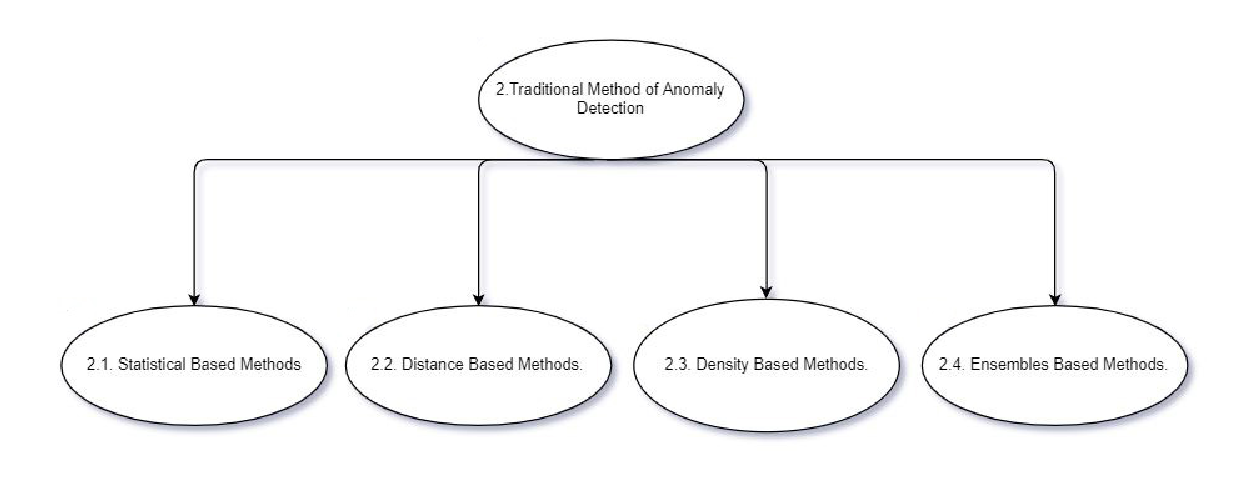
\includegraphics[width=0.80\textwidth]{figures/gif/secpictures/sec2}
%   \caption{Traditional Method of Anomaly Detection}\label{sec2}
% \end{figure}

\subsection{Statistical Based Methods}

The statistical based detection assumed that
if the difference between the data and the statistical
distribution or the specified model
is greater than a specific range~\cite{chandola2009anomaly},
the data object is considered as anomalier.
It include two special method:
distribution-based approach and
depth-based approach~\cite{wu2016survey}.

As for the distribution-based method,
after given a distribution,
a method of consistency checking is used to find anomalier.
However,
the actual distribution of the data set is always unknown,
and it is difficult to estimate the data distribution in high-dimensional.
To solve those problem,
self-organizing map (SOM)~\cite{siripanadorn2010anomaly},
Support Vector Regression~\cite{kromanis2013support} (SVR) and
other machine learning based methods are introduced to
improve those shortcomings.

The depth-based approach takes into account
that each object is a point with
a specified depth in n-dimensional space,
and that a data object may be anomalier with a lower depth.
Although some dimension reduction methods such as
Primary Component Analysis (PCA)~\cite{deng2013modified},
and Independent Component Analysis (ICA)
are commonly used in this category,
it still has a high computational complexity and
has a low efficiency in the big data with
high-dimensional and large data sets.

\subsection{Distance Based Methods}

\begin{figure}
  \centering
  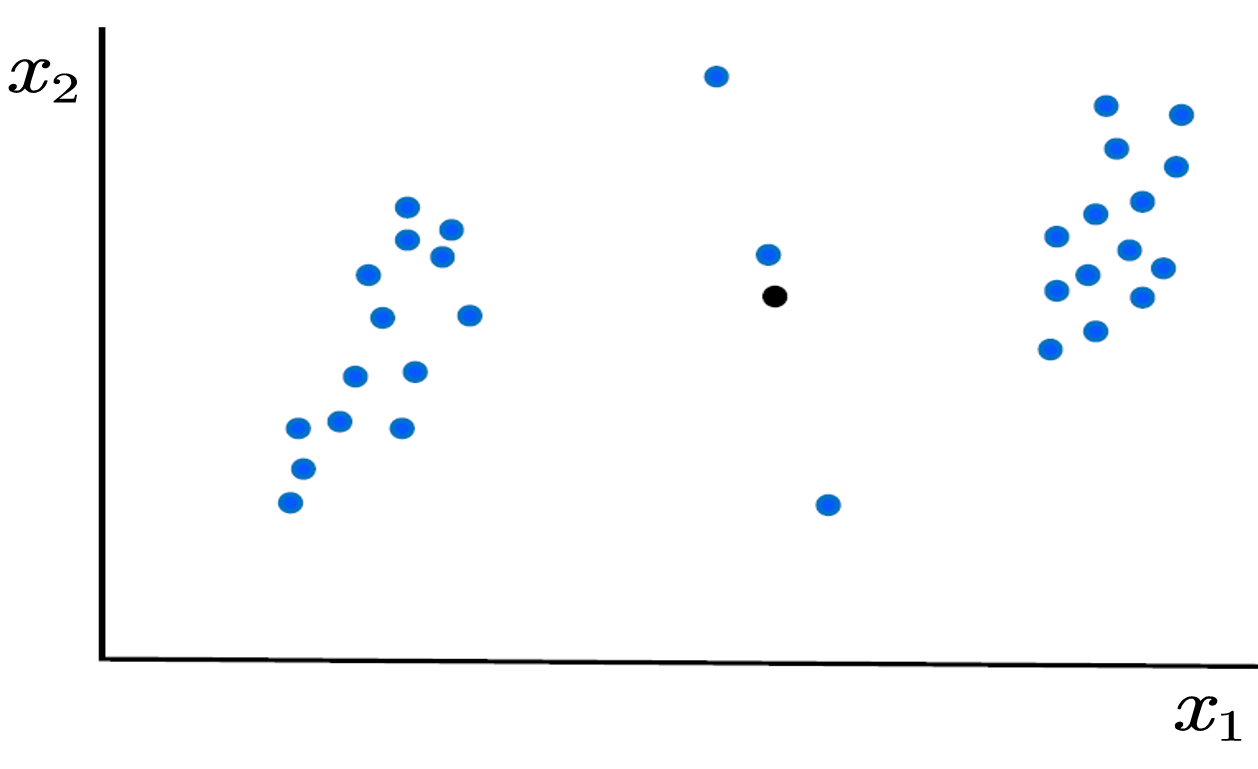
\includegraphics[width=0.8\textwidth]{figures/distance.png}
  \caption{Distance Based  Anomaly detection Methods}\label{fig:distance}
\end{figure}

The distance based anomaly detection
assumes that
anomaliers are far away from other points.
It calculate the distance between data points in
data space after setting a distance function.
A data object is regarded as anomalier when
the distance between itself and others is large.
The firstly anomaly detection method
based on distance is proposed in~\cite{knorr1997unified}.
Then it is extended to using K-neighbor distance to
build the anomaly detector~\cite{ramaswamy2000efficient,kuang2008anomaly}.
The K-neighbor distance of each object is calculated and
sorted from small to big,
the objects which have largest
distance are considered as anomaliers.

The distance based anomaly detection method
is easier to realize,
and is widely studied.
But the complexity of the algorithm is relatively high,
such as the computation complexity of KNN is $O(n^2)$,
where the $n$ is the number of data points.
and it cannot consider the size of
data sets and the scalability of data dimension.
%Secondly,
%it is pointed out distance based anomaly detection become invalid when
%the data sets has obvious internal density
%differences~\cite{breunig2000lof}.
%Its capability is not good in processing the data which
%contains a variety of distribution or
%are mixed with different densities subset.
%This is mainly because of the anomaly detection based on
%distance considers from all the viewpoints.
Thus the practical application of distance based methods is limited.

\subsection{Density Based Methods}
\begin{figure}
  \centering
  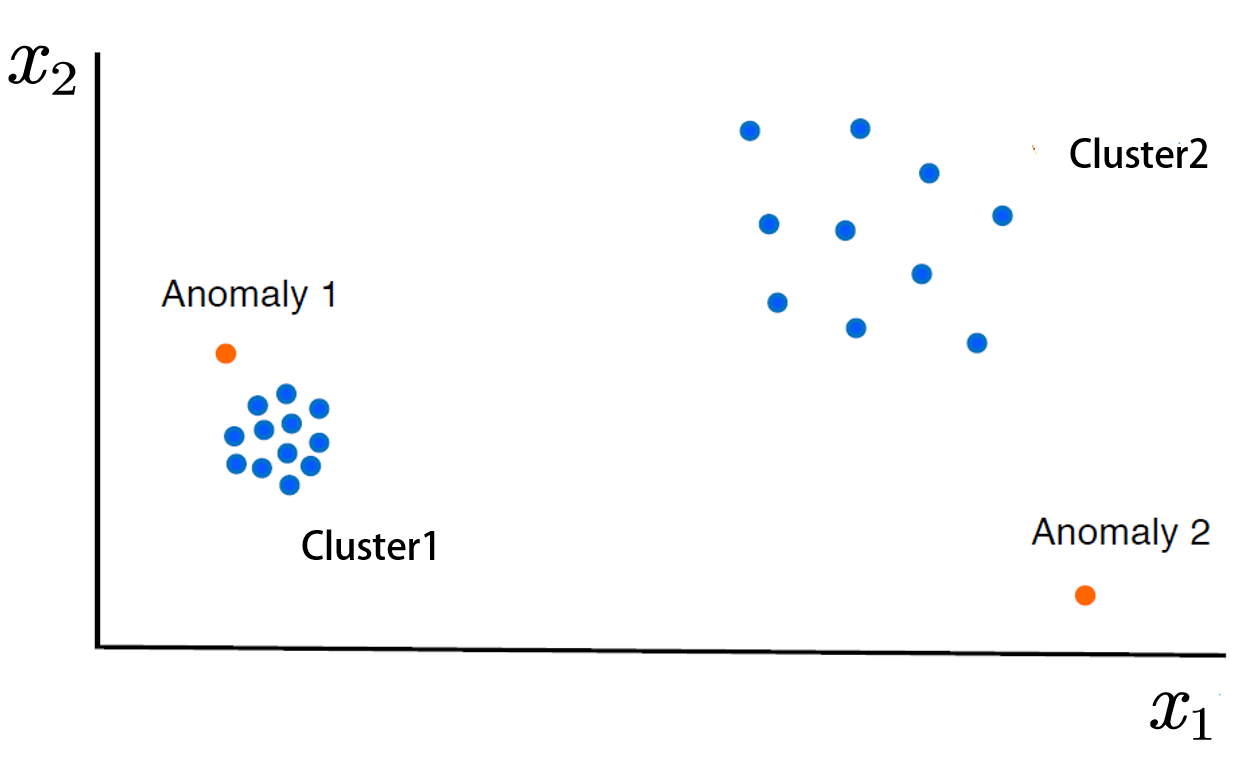
\includegraphics[width=0.8\textwidth]{figures/cluster.png}
  \caption{Density Based  Anomaly detection Methods}\label{fig:Density}
\end{figure}

%The statistical based and distance based methods have a common problem,
%that is,
%the overall distance criterion is used as the basis for the detection of anomaliers.
Anomaliers are usually detected from an individual's point of view,
i.e.
the anomaliers are far from their neighboring clusters.
Therefore,
it is not appropriate to use the overall distance as statistical based and distance based methods do.
The density-based anomaly detection algorithms are proposed to solve this problem.
The Local Outlier Factor (LOF)~\cite{breunig2000lof}
is proposed to detect anomaliers by comparing the local density of an object to the local density of its neighbors.
If the density of the data object is
much lower than that of its neighbors,
this data object is considered as anomalier.
Local parsimony factor (LCF) is proposed to
reduce the complexity of the
computation by considering the maximum distance between
the $k$ nearest objects as $k$ distances~\cite{agyemang2004algorithm}.
In addition,
multi-granularity deviation factor (MDEF) is used as a measure of anomaly which comparing the number of data objects in $r$ neighbors and their mean~\cite{papadimitriou2003loci}.
It does not need to calculate the density of the data points,
and the efficiency of the calculation is greater than LOF.

The density-based idea is closer to Hawkins' definition of
exception than the distance-based idea~\cite{hawkins1980identification}.
Therefore,
it can detect local anomaliers,
and have high detection accuracy.
However,
the time complexity is still very high,
and the result of detection is sensitive to
the selection of parameters such as the threshold of the outlier,
which is difficult to determine.

\subsection{Ensembles Based Methods}

Because each model is specifically designed
for different characteristics of perception.
It is only applicable to certain aspects of
the ``whole truth''.
So it is best to integrate different
third-party observational results to reach consensus.
The main idea of this method (called ``ensemble'')
is that if these judgments do not contain
all the same errors.
It is useful to combine individual judgments or
the results of marginalized observations~\cite{zhou2012ensemble}.
One would think that this is a majority vote of
the jury:
one or another judgment on the statement may be wrong,
but the majority judgment is still correct as long as
the judgment is generally reliable.
Isolation Forest~\cite{liu2008isolation}
can be treated as typical ensemble method,
it builds an ensemble of “Isolation Trees” (iTrees) for
the data set,
and anomaliers are the points that
have shorter average path lengths on the iTrees.
It has a low linear time complexity and
a small memory requirement
and is able to deal with high dimensional data 
with irrelevant attributes~\cite{chandola2009anomaly}.
FuseAD~\cite{munir2019fusead}
takes advantage of both statistical approach ARIMA
and deep-learning-based approach
CNN to propose an novel network:
it shows great improvement on Yahoo Webscope benchmark.
%However,
%we found that all the approaches mentioned above
%have no considerations for explanation of anomaly detection,
%and it is meaningful in practical process of industry.
%Therefore it is meaningful to put some works into use
%certain approach for explaning the  anomaly detection.

\section{Challenges of Anomaly detection in big data}
~\label{sec-challenge-big}
In the age of big data,
the design of anomaly detection methods have become increasingly complex.
The features of big data that have the greatest effect
on the anomaly detection and each 
feature has its individual challenges.
The Volume requires that 
the proposed method could effective detect anomaliers in large data set.
The Velocity brings challenges when data are increasing 
and arriving at speed as data streams.
These features make the anomaly detection method 
become highly complex and ineffective.
Here, 
we describe challenges of anomaly detection brought 
by each feature of big data and 
show the existing method to overcome them.
%We have described each one of them in the following subsections.

\subsection{Challenges in the Volume of big data}

When the potential probability distribution is not
known and the size of the data set is huge,
the computational requirements increase.
The Volume feature of big data emphasizes storage,
memory,
and computing power of the system to
cope with ever-increasing data size~\cite{gadepally2014big}.
When the data size is large,
the traditional anomaly detection methods may become invalid,
because of the limited computational power and associated factors.
To overcome this issue,
several parallel and distributed computing methods are proposed.

Managing computational power and disk input/output (I/O) communication can
improve the efficiency of the method.
D-cube~\cite{shin2017d} is a disk-based detection method to
find fraudulent lockstep behaviour in large scale data and
runs in a distributed manner across multiple machines.
It is proved that could successfully
detect network attacks and
synchronised behaviour in rating data
with highest accuracy.
Nested loop (NL)\cite{knox1998algorithms} is
a straightforward method to detect anomaliers in a database.
Hung and Cheung~\cite{hung2002parallel} introduced an
efficient and parallel version
of the NL algorithm that reduces both computation and disk I/O costs.

Ramaswamy et al.~\cite{ramaswamy2000efficient} proposed a
distance based  anomaly detection method to detect anomalier in huge data sets.
It segregates input data into
separate subsets and prunes partitions that
do not contain anomaliers,
resulting in considerable
savings in computation.
DOLPHIN ~\cite{angiulli2007very} is also a
distance based anomaly detection method
that works on disk-resident data sets in huge datasets.

To solve the sequential exception problem in large databases,
Arning et al.~\cite{arning1996linear} proposed a linear algorithm
using a dissimilarity function to capture the
similarity rate of a data point.
Erfani et al.~\cite{erfani2016high} introduced
an unsupervised method for high-dimensional large-scale
unlabeled data sets to detect anomaliers that
are a combination of a deep belief network (DBN) and one-class
support vector machines (SVM).
One-class SVMs (1SVMs) are used for detecting anomaliers
through unsupervised learning and aim to
model the underlying distribution of data while
not considering irrelevant attributes or
anomaliers in the training records.
Features derived from training samples are taken as input to train 1SVMs.
Conversely,
a DBN is
a multiclass semi-supervised approach and dimensionality reduction tool.
It uses multilayer
generative models (non-linear manifold) that learn one layer of features at a time
from unlabeled data.
% Camacho et al.~\cite{camacho2014tackling} presented an interesting outline for anomaly
% detection,
% identifying and interpreting unusual events in a forensics system network by addressing the 4Vs of big data—volume,
% variety,
% veracity,
% and velocity.
% Their framework
% is based on input from several heterogeneous data sources.
% First,
% the system pre-processes
% incoming data;
% second,
% extracted features are calculated from the streaming data;
% third,
% all features representing diverse sources are
% combined and called a parameterizations
% step;
% and,
% fourth,
% these new features are utilized in updating a set of intermediate
% data structures representing the present stage of the network.
% The updated strategy follows
% an exponentially weighted moving average method and uses a PCA model.


\subsection{Challenges in the Velocity of big data}

Most traditional anomaly detection methods assume that
the data set is generated
by an unknown but stationary probability distribution
,
the volume of data is finite and
the entire dataset could be stored for analysis~\cite{silva2013data}.
However,
in the big data age,
the data set would be
an infinite set of data instances in which
each instance is a
set of values with an explicit or
implicit time stamp
and it is refered as data stream~\cite{sadik2014research}.
The data stream are unbounded
sequences and the entry rate is continuously high,
as the respective variations repeatedly
change over time.
The anomaly detection on data stream,
as show in Figure~\ref{fig:streamAnomaly},
is a highly challenge tasks because of
the unbounded volume of data,
the high rate of data generation,
and data be stored will run out of memory space~\cite{sadik2014research}.

\begin{figure}
  \centering
  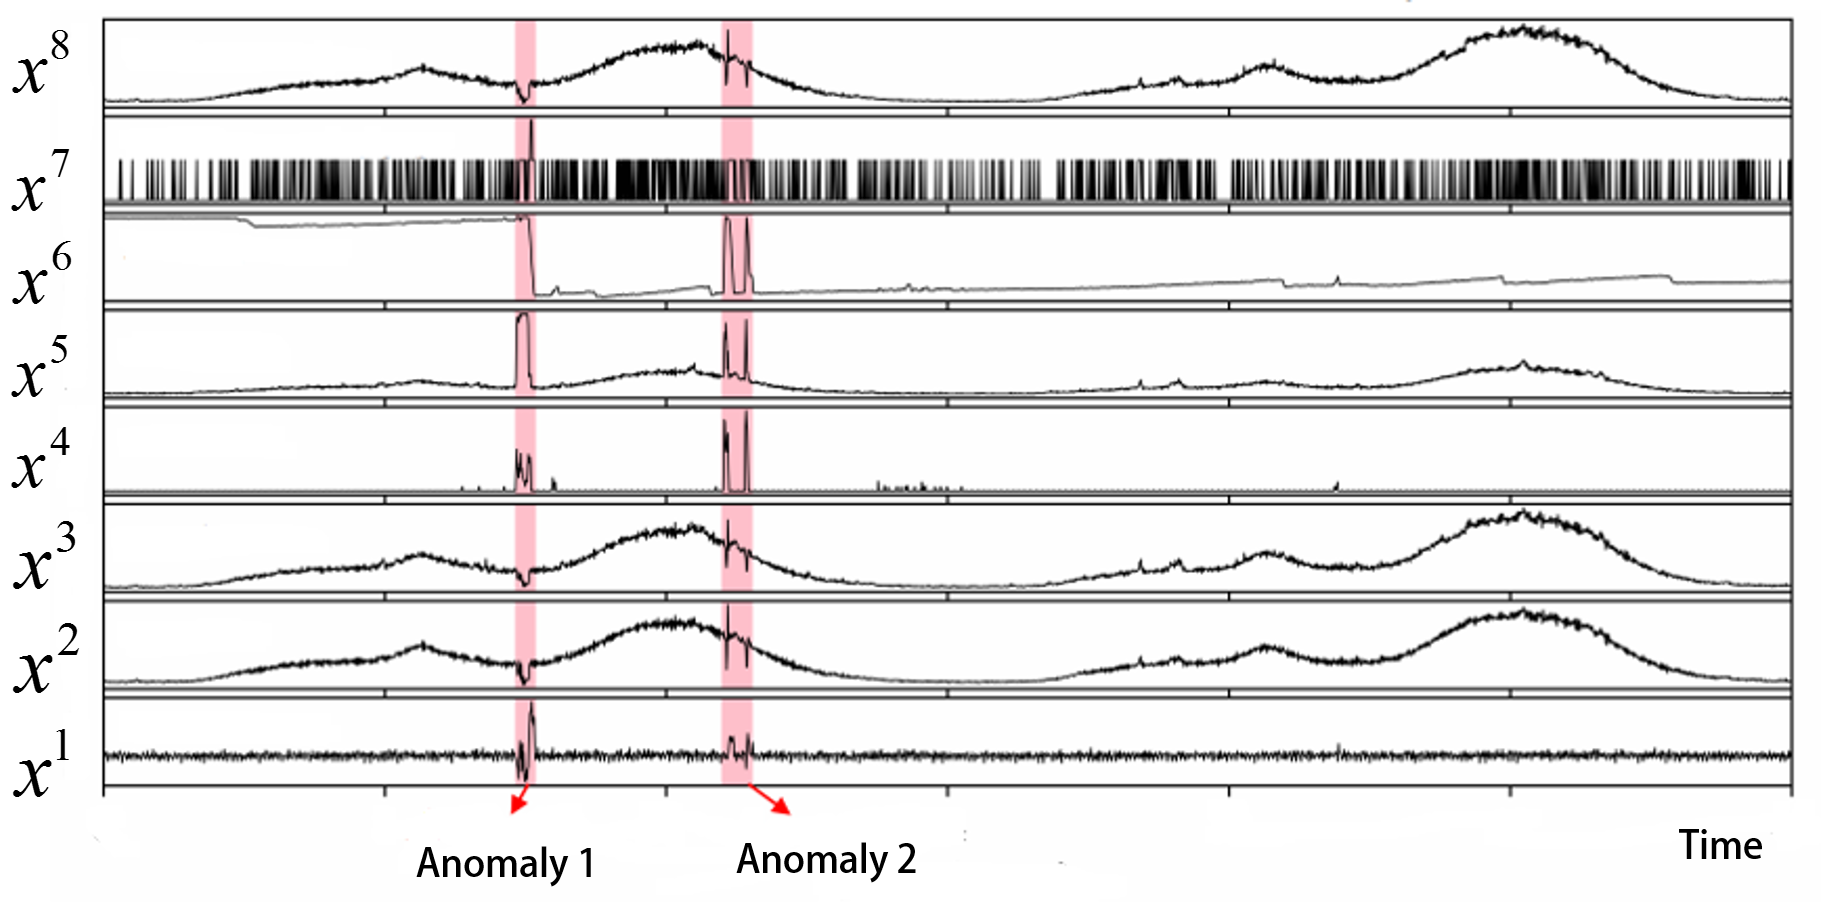
\includegraphics[width=0.8\textwidth]{figures/streamAnomaly.png}
  \caption{Anomaly detection on stream data}\label{fig:streamAnomaly}
\end{figure}

In most data stream scenarios,
more recent information from the stream can reflect the
emerging of new trends or changes on the data distribution.
% This information can be
% used to explain the evolution of 
% the process under observation.
Most method use the sliding-window model to 
capture this feature of data stream.
In the the sliding-window model.
only the data which from the current period of time 
up to a certain period in the past
are stored in a data structure 
where the window size can be variable
or fixed.
This data structure is usually a first in,
first out (FIFO) structure i.e. first object added will be the first one to be removed,
An example of the sliding-window model is presented in Figure~\ref{fig:slidingWindow}.
\begin{figure}
  \centering
  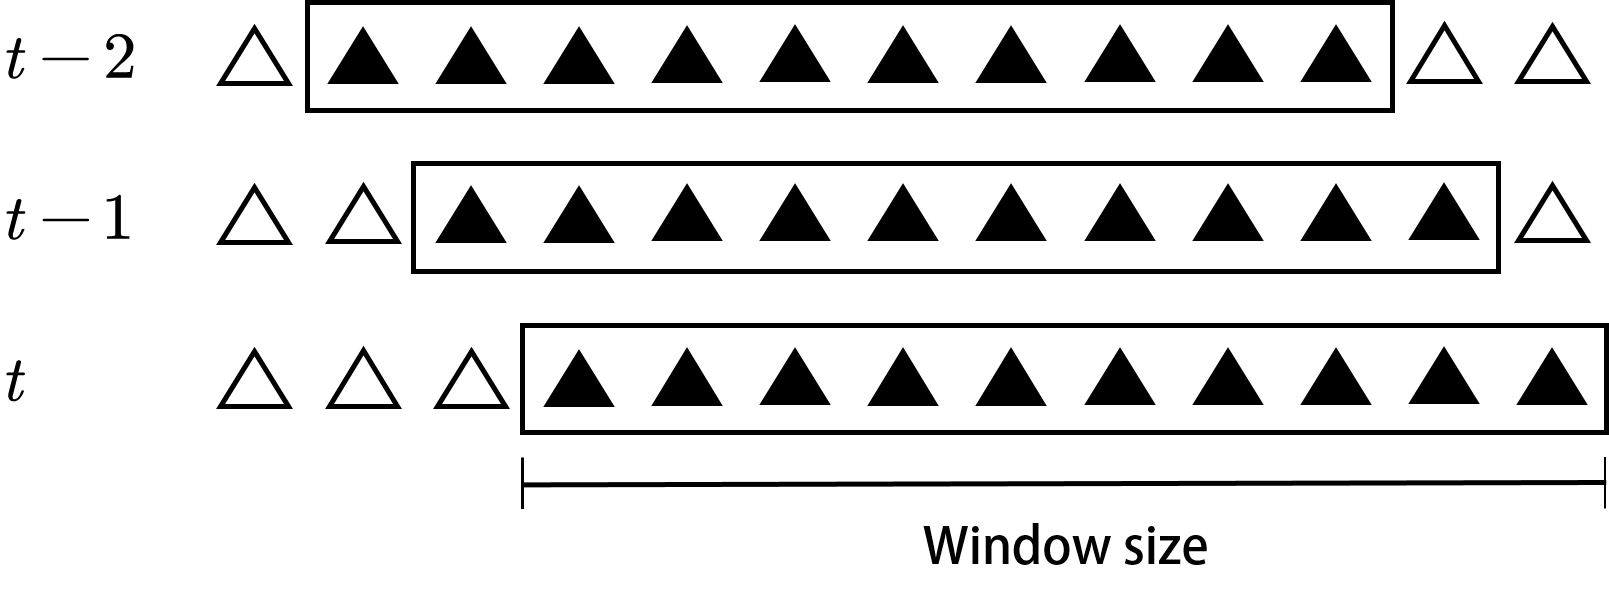
\includegraphics[width=0.8\textwidth]{figures/slideWindow.png}
  \caption{Sliding window model}\label{fig:slidingWindow}
\end{figure}
% Data streams reflect the important features of big data in that the
% aspects of both volume and velocity are temporally ordered,
% evolving,
% and potentially
% infinite.


% Data streams are ,
% which makes the task of detecting anomaliers and extracting useful insights
% challenging.
% This is a main disadvantage that arises in several application areas~\cite{salehi2016fast}.
%Silva et al.~\cite{silva2013data} summarized
%the following challenges should be considered for developing
%a successful anomaly detection methods in data streams:
%\begin{inparaenum}
%  \item the data instances arrive continuously;
%  \item there is no control over the order of processing or
%  handling of data instances;
%  \item the
%  size of a data stream can be unbounded;
%  \item data instances are deleted after processing;
%  and
%  \item the data generation process can be nonstationary;
%  hence,
%  its probability
%  distribution may evolve over the period.
%\end{inparaenum}
% The data may comprise irrelevant attributes that
% raise problems for anomaly detection,
% and there are several other factors involved,
% such as whether the data are from
% a single source or multiple sources.
% Multiple data streams are made up of a set of data
% streams,
% and every data stream comprises an infinite
% sequence of data instances accompanied
% by an explicit or implicit time stamp history.
% In a single data stream,
% anomaly
% detection compares the history of data instances to
% determine whether an instance is an
% outlier or anomaly.
% By contrast,
% in multiple data streams,
% data instances are recognized
% as anomaliers by comparing them to
% the history of data instances from the same stream
% or other streams.

% A hypothesis behind all data stream models is that
% the most recent data instances
% are more than historical data.
% The simplest model uses sliding windows of fixed size
% and works on the basis of first in,
% first out~\cite{gama2012survey}.
% A sequence-based sliding window
% is one in which the size of the window is defined
% as the number of observations in
% regard to fixed size and specific time~\cite{pettis1979intrinsic}.
% There is another type of sliding window
% called a time stamp window in which
% the size of the window is representative of the
% duration of the data~\cite{gama2012survey}.

Angiulli and Fasseti~\cite{angiulli2007detecting}
introduced methods for recognizing distance-based
anomaliers in data streams using a sliding window model in which
anomaly queries are executed for the purpose of
identifying anomaliers in the current window.
Their algorithms
execute anomaly queries and return an approximate answer based on accurate
estimations with a statistical guarantee.
These algorithms are based on a method
known as stream outlier miner,
or STORM,
which is used to find anomaliers on distance based
windowed data streams.
A sliding window is used to continuously inspect the
object until it expires.
% Later,
% Angiulli and Fasseti~\cite{angiulli2009detecting} presented
% an additional algorithm for identifying distance-based anomaliers
% in data streams using the sliding window
% model; although based on their previous approximate algorithm,
% this algorithm
% emphasized fixed memory requirements.

An algorithm based on the sliding window model for
mining constrained frequent
item sets on uncertain data streams was introduced by
Yu et al.~\cite{yu2016uncertain}.
Known as CUSFgrowth
(constrained uncertain data stream frequent item sets growth),
the algorithm
determines the order of items in transactions and
analyzes the properties of constraints.
According to the order of items determined by
the properties of constraints a CUSF-tree
is created; later,
after the frequent item sets are satisfied,
the constraints are mined from
the CUSF-tree.

% Kontaki et al.~\cite{kontaki2011continuous}
% also studied the problem of continuous anomaly detection in
% data streams using sliding windows.
% They proposed four algorithms that sought effective
% anomaly monitoring with lesser memory requirements.
% Apart from assuming that the
% data are in metric space,
% their model did not make any assumptions about
% the behavior of input data.
% Their methods have considerable flexibility with
% regard to parameter values,
% enabling the execution of multiple distance-based
% anomaly detection tasks
% with different values,
% and they reduced the number of distance computations using
% micro-clusters.
% Their primary concerns were to improve efficiency and
% reduce storage
% consumption.
% Their methods incorporate an event-based framework that bypasses
% unneeded computations benefiting from the expiration time of objects.

In addition,
enseble-based methods are also proposed to
resolve the problem of detecting anomaliers
in streaming data.
iForestASD~\cite{ding2013anomaly},
uses sliding window to deal with streaming
data.
On the current complete window,
iForestASD uses the standard
iForest method to to adapte streaming
data anomaly detection.
% A continuous outlier detection algorithm (CODA) is
% an event-based method that
% estimates the expiration time of objects to
% circumvent undesirable computations.
% This method quickly determines the nature of elements
% by probabilistic pruning,
% thereby improving efficiency and
% consuming significantly less storage.
% Since different users may
% have different views of anomaliers,
% an advanced CODA that can handle numerous values by
% enabling the concurrent execution of various
% monitoring strategies has also been proposed.
% Another algorithm to decrease
% the quantity of distance computations—microcluster
% CODA—was inspired by the work of Zhang et al~\cite{tian1996efficient}.
% Explaining anomaly detection is the task of making
% the anomaly detection process more transparent to the users,
% i.e. why are these samples are recorded as anomaliers?
% % The Explaining anomaly detection task refers to
% % making users fully understand the anomaly behavior.
% % However,
% The  goal of explanation is not only to
% convince the users about the proposed anomoaly detection method,
% but also helping the users to understand behavior about
% the anomaliers.
% This process will help the users to make decision such as
% adjusting some feature of sample according to propsed method to
% make the anomalier to normal.

% Over the last decade,
% several methods have been developed to explain the models.
% One method consists of using an approximate approximation of
% the original model~\cite{lundberg2017unified}.
% Examples of interpretive approximation methods using
% the original model:
% LIME~\cite{ribeiro2016should}
% (this is an example of a model-independent method
% used to explain predictions using local models) and
% DeepLIFT~\cite{shrikumar2017learning}
% (used to explain local models Example).
% A model-specific method for interpreting deep learning models
% in which the contribution of all neurons in the network is
% propagated back to the input properties.
% SHAP - SHapley Additive exPlanation ~\cite{lundberg2017unified} uses
% Shapley value in game theory to ensure feature consistency combined
% with previous methods and
% interprets predictions by calculating the importance of features.

% Most of the existing works focus on mining anomalying features to
% produce the subspaces where
% the anomaliers exhibiting most abnormality.
% Dang et al.~\cite{dang2013local} introduced LODI to
% seek an optimal subspace where
% the distance between an anomaliers and
% inliers can be maximized.
% Micenkova et al.~\cite{micenkova2013explaining}
% defined separability through the classification error of anomaliers and
% inliers,
% and leveraged it to
% quantify the explanation within every subspace.
% Then,
% they compared the measured explanations and
% selected the most explanatory subspace as the explanation of the anomaliers.
% LOGP is proposed ~\cite{dang2014discriminative}  to
% conduct a graph projection on anomaliers,
% which would further sort out the abnormal subspaces as the explanation.
% Duan et al. ~\cite{duan2015mining}
% demonstrated OAMiner,
% which focused on efficient mining of the discriminative subspaces.
% Macha et al.~\cite{macha2018explaining}
% demonstrated a pattern discover method providing explanations represented as hyper-ellipsoids.
% They conducted a clustering operation based on the density and
% purity of the involved instances before searching for the explanations.
% Then,
% several other literatures further derived rules to
% illustrate the deviation between anomaliers and
% inliers.
% Muller et al.~\cite{muller2012outrules}
% introduced OutRules to
% find normal and abnormal features and
% produce rules indicating the deviating behavior of anomaliers.
% He et al.~\cite{he2010co}
% demonstrated a method co-selecting the features and
% relevant anomaliers to
% describe the differences with inliers.

\section{Evaluation of Anomaly Detection}~\label{sec:evaluate}
Evaluation metrics are critical to building a
successful anomaly detection system.
Efforts have been made to determine the
correct method for measuring the quality of abnormal detection.
This section examines general evaluation metrics from two aspects:
supervised detection
and unsupervised detection which is
distinguished by whether have labeled dataset.

\subsection{Supervised Evaluation}
When the ground truth of dataset is valuable,
the supervised evaluation method could be used.
The most popular supervised evaluation method
are accuracy, 
recall,
F1 score,
ROC curve,
and AUC.

\subsubsection{Confusion Matrix}
The confusion matrix,
as shown in Table~\ref{tb:confusion},
is a table two dimensions
where each row of the matrix represents the instances
in a predicted class while
each column represents the instances
in an actual class~\cite{powers2011evaluation}.
TP means true positives
(i.e. items correctly labeled as belonging to the positive
class),
FP means false positives
(i.e. items incorrectly labeled as belonging to the
positive class),
FN means false negatives
(i.e. items which were not labeled as
belonging to the positive class but should have been).
TN means true negative
(i.e. items correctly labeled as belonging to the negative
class).

\begin{table}  \centering
  \caption{Confusion Matrix.
  TP is True Positive;
  FP is False Positive;
  TN is True Negative;
  FN is False Negative. }
  \label{tb:confusion}
  \begin{tabular}{ccc}
  \toprule
    & Actual value   &  Actual value    \\
  \midrule
  Predicted value  & TP & FP  \\
  Predicted value    & FN & TN  \\
  \bottomrule
  \end{tabular}
\end{table}


\subsubsection{Precision}

The \textit{Precision} measures the ratio of
examples classied as positive that
are truly positive~\cite{ting2010precision}.

\begin{equation}
  precision=\frac{TP}{TP+FP}
\end{equation}

\subsubsection{Recall}
The \textit{Recall} measures the ratio of positive examples that
are correctly labeled.

\begin{equation}
  recall=\frac{TP}{TP+FN}
\end{equation}

\subsubsection{F1 Score}
The \textit{F1 score} is a tradeoff between
the \textit{Precision} and \textit{Recall}:
\begin{equation}
  F1=\frac{2*precision*recall}{precision+recall}
\end{equation}
F1 metric weights recall and
precision equally,
and a good detection algorithm will
maximize both precision and
recall simultaneously.
Moderately good performance on
both will be favored over
extremely good performance on
one and poor performance on the other.

%\subsubsection{ROC Curve}
\subsubsection{AUC}
\textit{AUC} (area under curve) refers to the area under the \textit{ROC curve}.
The vertical and horizontal axis ranges are (0,1),
so the total area is less than 1~\cite{bradley1997use}.
The larger the \textit{AUC},
the better the classification effect.

The \textit{AUC} value can be think as the probability that
the two randomly selected objects (positive example (anomalier)
and negative example (normalier)) are arranged correctly
(i.e.,
anomalier is classified before the normalier value)~\cite{hanley1982meaning}.
The \textit{ROC curve} and \textit{AUC}
analysis inherently address the problem of imbalance using
relative frequencies,
making them particularly popular in evaluating
the detection of exclusion.

\subsection{Unsupervised Evaluation}
If some tasks of anomaly detection  
have no ground truth,
the unsupervised evaluation method
such as comparative evaluation,
generating pseudo tags,
and similarity analysis can be used.

\subsubsection{Comparative Evaluation}

For unsupervised learning,
a common evaluation strategy is to rank the
results according to the score of anomaliers,
and then iteratively set the threshold from
the first to the last.
This will form n ancestor values
(true positive rate and false positive rate),
and a ROC curve can be obtained.
The integral AUC of ROC can be used as a measure
to test the performance.


\subsubsection{Generating Pseudo Tags}

There are a lot of learning efforts to transform
unsupervised learning into supervised learning,
and there are now feasible methods.
Then,
we can use the evaluation methods of supervised learning,
such as accuracy.

\subsubsection{Similarity Analysis}

Unsupervised learning often depends
on the similarity between data,
which can be expressed as spatial density
or distance measurement.
In the evaluation of anomaly detection algorithm,
it can be assumed that a large number of normal
data are closely adjacent (can form multiple clusters),
and anomaliers are often quite different from these normal points.

\section{Anomaly detection software packages}~\label{sec:tools}
Many companies have build
their own anomaly detection systems in order to
meet their specific business needs.
However,
there are still many open source anomaly detection packages available.
In this section,
we review some of the popular software packages for
practitioners to build their anomaly detection systems.

\subsection{PyOdds}

PyODDS (\href{http://pyodds.com/}{http://pyodds.com/})
is an end-to end Python system for
anomaly detection.
It provides several anomaly detection algorithms and
support both static and time-series data type.

\subsection{PyOD}
PyOD~\cite{zhao2019pyod} (\href{https://pypi.org/project/pyod/}{https://pypi.org/project/pyod/})
is a comprehensive and scalable Python toolkit for
detecting anomalier in multivariable data.
It includes more than 20 detection algorithms,
including new deep learning models and ensembles methods.

% \subsection{Anomaly Detection Toolbox}
% Anomaly Detection Toolbox
% (\href{http://dsmi-lab-ntust.github.io/AnomalyDetectionToolbox/}{http://dsmi-lab-ntust.github.io/AnomalyDetectionToolbox/})
% collectes a lot of popular anomaly detection algorithms in Matlab.

\subsection{ADTK}
Anomaly Detection Toolkit (ADTK) (\href{https://adtk.readthedocs.io}{https://adtk.readthedocs.io})
is a Python package for unsupervised / rule-based time series anomaly detection.

\subsection{Scikit-Multiflow}
Scikit-Multiflow~\cite{montiel2018scikit}
is the main open source machine learning framework
for multi-output,
multi-label and data streaming.
Implemented in Python language,
it includes various algorithms and
methods for streams mining.

\subsection{Distributed Computing frameworks}
Distributed computing is one of the most
important techniques to handle big data.
Many frameworks for distributed computing
such as Apache Hadoop
(\href{https://hadoop.apache.org/}{https://hadoop.apache.org/}),
Apache Spark
(\href{https://spark.apache.org/}{https://spark.apache.org/}),
and Apache Flink
(\href{https://flink.apache.org/}{https://flink.apache.org/})
were developed to address the challenges of big data.
Most of these frameworks
have in-house machine learning (ML) libraries to build 
the application of anomly detecion.


% \subsection{RRCF}
% RRCF~\cite{bartos_2019_rrcf} (\href{https://travis-ci.org/github/kLabUM/rrcf}{https://travis-ci.org/github/kLabUM/rrcf})

\section{Conclusions} \label{sec-conclusions}

Anomoaly detection has been extensively
attentted in recent years in the modern industry.
This chapter aimed to present the state of the art
anomaly detecttion for practical using in industry.
This has included anomoaly detection method based on distribution,
distance,
density,
cluster and ensemble.
To evaluate anomoaly detection method,
we reviewed commonly used
two categories including supervised and unspervisd.
In addition,
we reviewd the explanation of anomoaly detection which
has been getting more and more attention.
Finaly,
we provided a list of free and open source software packages for
practitioners to create their own anomaly detection systems.

A wide range of studies have been carried out in the field of abnormal detection.
As this chapter only coveres this topic,
we recommend reader to read more detail in the references of this chapter.


% \blindtext

% % %\section*{Acknowledgment}

% % \lipsum[1]


% % The authors would like to thank \ldots
